\section{Anexo I: Encuesta evaluativa}
\label{AnexoI}
\begin{enumerate}

\item ¿Sexo?: \\

$\bigcirc$ Masculino \\
$\bigcirc$ Femenino

\item Rango de edad: \\

$\bigcirc 10 - 17$\\
$\bigcirc 18 - 24$\\
$\bigcirc 25 - 32$\\
$\bigcirc 33 - 39$\\
$\bigcirc 40 - $o más

\item ¿Está al tanto de lo que es ``{\gam}/ludificación'' ? \\

$\bigcirc$ Si \\
$\bigcirc$ No

\item ¿Usted acumula puntos de grandes empresas?\\

$\bigcirc$ Si \\
$\bigcirc$ No    

\item  (Si contesto ``No'' en la pregunta anterior, pasar a la pregunta 7.) En empresas donde sea socio o participe acumulando puntos, ¿Está al tanto de los beneficios que dicha empresa le ofrece?\\

$\bigcirc$ Si \\
$\bigcirc$ No

\item ¿Ha utilizado éstos beneficios en algún momento?\\

$\bigcirc$ Si \\
$\bigcirc$ No

\item Al momento de comprar, ¿Qué beneficios prefiere o preferiría obtener?:

\begin{table}[h]
\centering
\begin{tabular}{|l|c|c|c|c|c|}
\hline
 & {\bf 1} & {\bf 2} & {\bf 3} & {\bf 4} & {\bf 5} \\
\hline
Precios bajos. & $\bigcirc$ & $\bigcirc$ & $\bigcirc$ & $\bigcirc$ & $\bigcirc$ \\
\hline
Acumulación de puntos. & $\bigcirc$ & $\bigcirc$ & $\bigcirc$ & $\bigcirc$ & $\bigcirc$ \\
\hline
Descuentos en próximas compras. & $\bigcirc$ & $\bigcirc$ & $\bigcirc$ & $\bigcirc$ & $\bigcirc$ \\
\hline
Obtención de productos exclusivos. & $\bigcirc$ & $\bigcirc$ & $\bigcirc$ & $\bigcirc$ & $\bigcirc$ \\
\hline
Reconocimiento publico según tabla de posiciones. & $\bigcirc$ & $\bigcirc$ & $\bigcirc$ & $\bigcirc$ & $\bigcirc$ \\
\hline
\end{tabular}
\end{table}

\item ¿Cuál es su preferencia a la hora de realizar compras? \\

$\bigcirc$ Presencial (persona a persona) \\
$\bigcirc$ On-line (vía internet)

\item Teniendo en cuenta lo que consiste ``{\gam}'', ¿Prefiere un sitio de ventas on-line con ``{\gam}'' o un sitio convencional? \\

$\bigcirc$ Tienda on-line con {\gam} \\
$\bigcirc$ Tienda on-line convencional

\item ¿Cree usted que el uso de ``{\gam}'' lo motiva para volver a comprar en la tienda? \\

$\bigcirc$ Si \\
$\bigcirc$ No

\item  ¿En que contexto estaría dispuesto al uso de ``{\gam}''?(Puede responder más de una)\\
 
$\bigcirc$ Trabajo. Ej. Reconocimiento y motivación mediante el uso de una tabla de posiciones asociada a la productividad. \\
$\bigcirc$ Educación. Ej: Entrega de beneficios por tareas completadas. Estos beneficios pueden ser la utilización de puntos para poder cambiar preguntas de una prueba por otra. \\
$\bigcirc$  Social. Ej: Conectar con personas para obtener beneficios mutuos. Un tipo de beneficios es descuentos al invitado y al que hizo la invitación luego de la primera compra del invitado.
\end{enumerate}

\section{Anexo II: Graficos }

\begin{figure}[!htb]
    \centering
    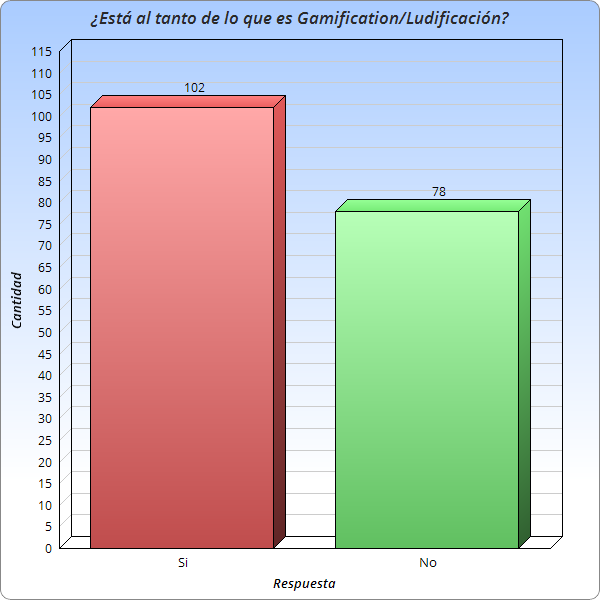
\includegraphics[width=0.6\textwidth]{images/Graficos/graf_5_1.png}
    \caption[chart5.1]{Respuesta a pregunta $3$, conocimiento de {\GAM}.}
    \label{fig:chart5.1}
    %\url{http://www.chartgo.com/get.do?id=69b1dc7d4e}
\end{figure}

\begin{figure}[!htb]
    \centering
    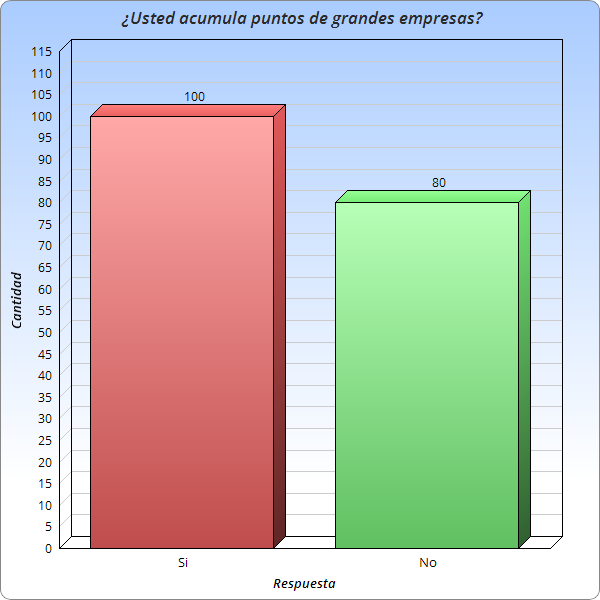
\includegraphics[width=0.6\textwidth]{images/Graficos/graf_5_2.png}
    \caption[chart5.2]{Respuesta a pregunta 4, acumulación de puntos.}
    \label{fig:chart5.2}
    %\url{http://www.chartgo.com/get.do?id=69b1dc7d4e}
\end{figure}

\begin{figure}[!htb]
    \centering
    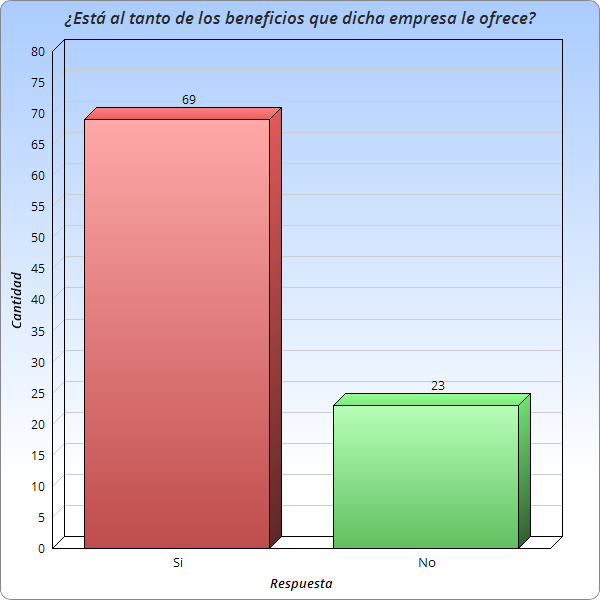
\includegraphics[width=0.6\textwidth]{images/Graficos/graf_5_3.png}
    \caption[chart5.3]{Respuesta a pregunta 5, conocimiento de beneficios.}
    \label{fig:chart5.3}
    %\url{http://www.chartgo.com/get.do?id=69b1dc7d4e}
\end{figure}

\begin{figure}[!htb]
    \centering
    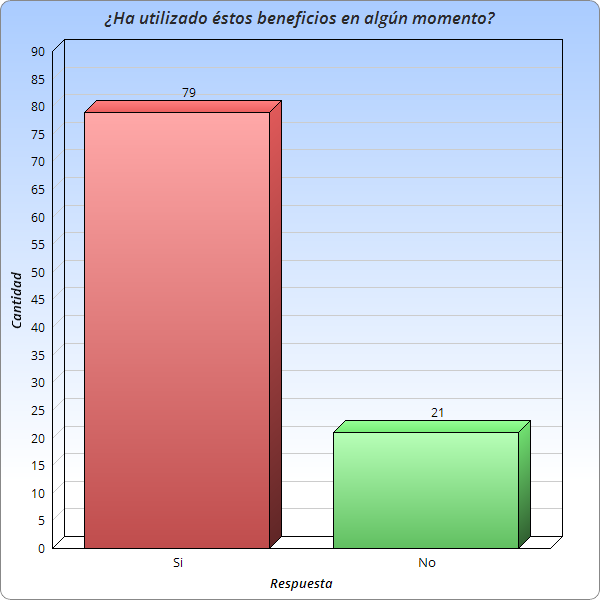
\includegraphics[width=0.6\textwidth]{images/Graficos/graf_5_4.png}
    \caption[chart5.4]{Respuesta a pregunta 6, utilización de los beneficios.}
    \label{fig:chart5.4}
    %\url{http://www.chartgo.com/get.do?id=69b1dc7d4e}
\end{figure}

\begin{figure}[!htb]
  \centering
  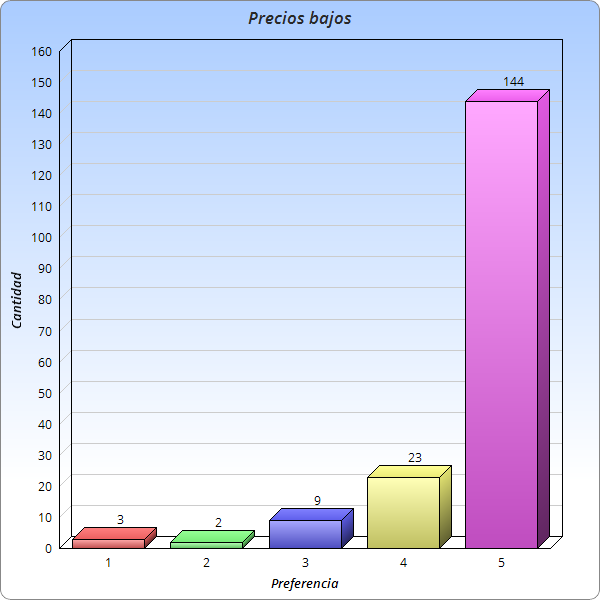
\includegraphics[width=0.6\textwidth]{images/Graficos/graf_5_5.png}
  \caption[chart5.5]{Respuesta a pregunta 7, cantidad de preferencias a beneficio de precios bajos.}
  \label{fig:chart5.5}
  %\url{http://www.chartgo.com/get.do?id=69b1dc7d4e}
\end{figure}

\begin{figure}[!htb]
  \centering
  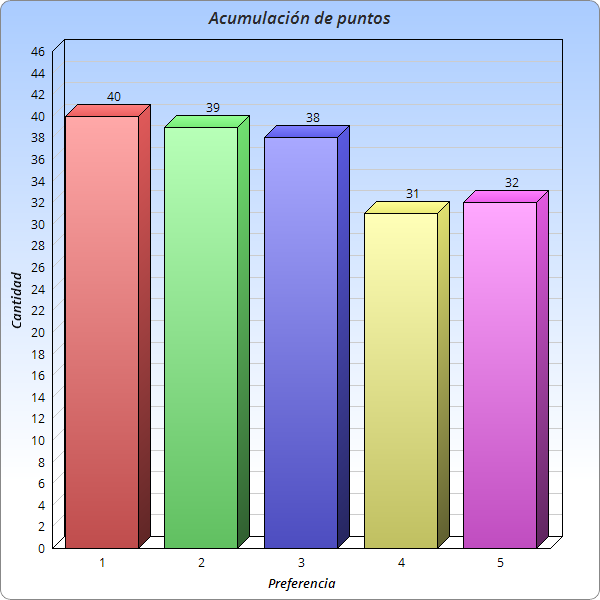
\includegraphics[width=0.6\textwidth]{images/Graficos/graf_5_6.png}
  \caption[chart5.6]{Respuesta a pregunta 7, cantidad de preferencias a beneficio de acumulación de puntos.}
  \label{fig:chart5.6}
  %\url{http://www.chartgo.com/get.do?id=69b1dc7d4e}
\end{figure}

\begin{figure}[!htb]
  \centering
  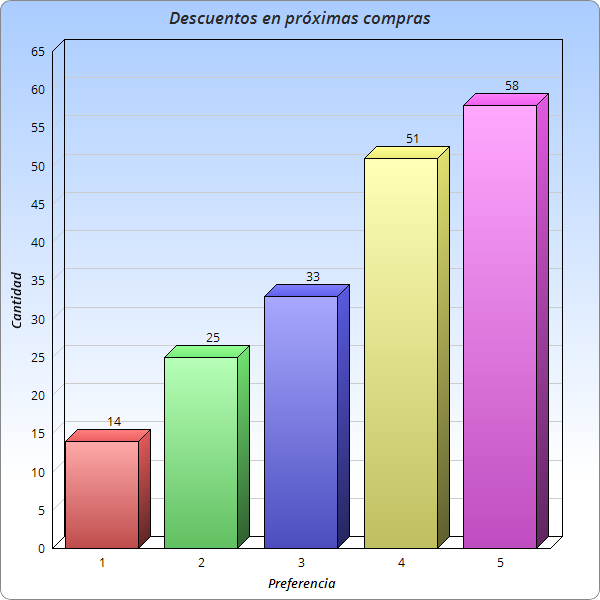
\includegraphics[width=0.6\textwidth]{images/Graficos/graf_5_7.png}
  \caption[chart5.7]{Respuesta a pregunta 7, cantidad de preferencias a beneficio de descuento en
próximas compras.}
  \label{fig:chart5.7}
  %\url{http://www.chartgo.com/get.do?id=69b1dc7d4e}
\end{figure}

\begin{figure}[!htb]
  \centering
  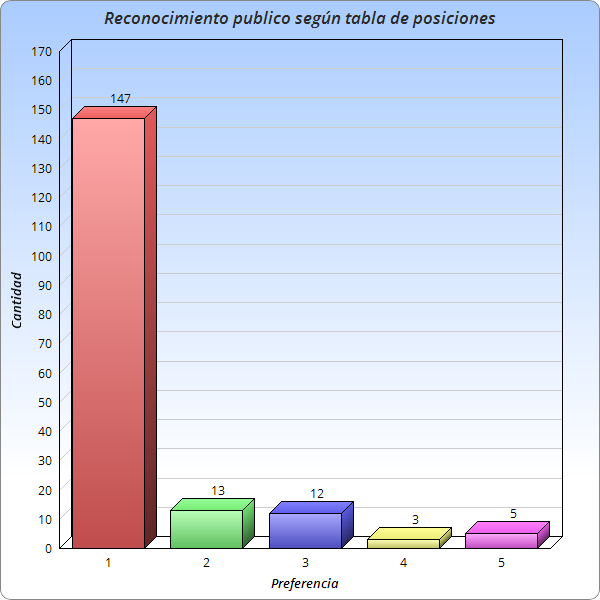
\includegraphics[width=0.6\textwidth]{images/Graficos/graf_5_8.png}
  \caption[chart5.8]{Respuesta a pregunta 7, cantidad de preferencias a beneficio de reconocimiento
publico según tabla de posiciones.}
  \label{fig:chart5.8}
  %\url{http://www.chartgo.com/get.do?id=69b1dc7d4e}
\end{figure}

\begin{figure}[!htb]
  \centering
  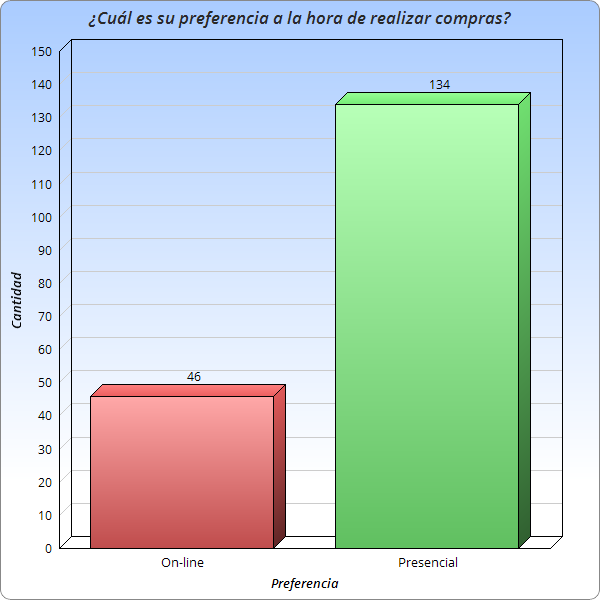
\includegraphics[width=0.6\textwidth]{images/Graficos/graf_5_9.png}
  \caption[chart5.9]{Respuesta a pregunta 8, preferencia al momento de comprar.}
  \label{fig:chart5.9}
  %\url{http://www.chartgo.com/get.do?id=69b1dc7d4e}
\end{figure}

\begin{figure}[!htb]
  \centering
  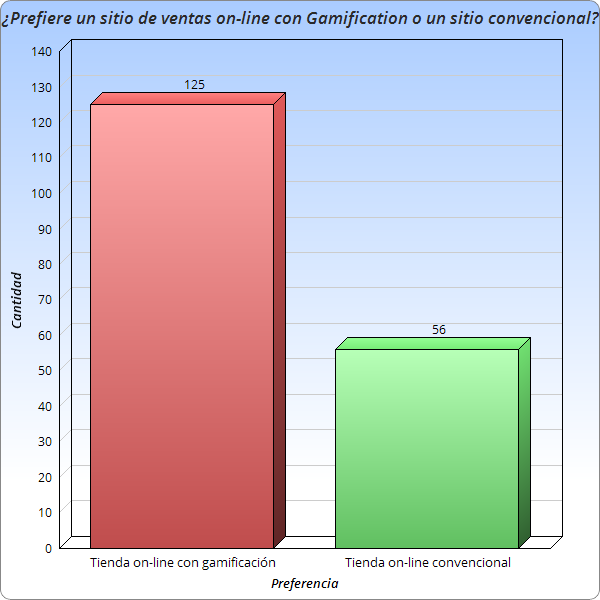
\includegraphics[width=0.6\textwidth]{images/Graficos/graf_5_10.png}
  \caption[chart5.10]{Respuesta a pregunta 9, preferencia al momento de comprar de forma \emph{on-line}.}
  \label{fig:chart5.10}
  %\url{http://www.chartgo.com/get.do?id=69b1dc7d4e}
\end{figure}

\begin{figure}[!htb]
  \centering
  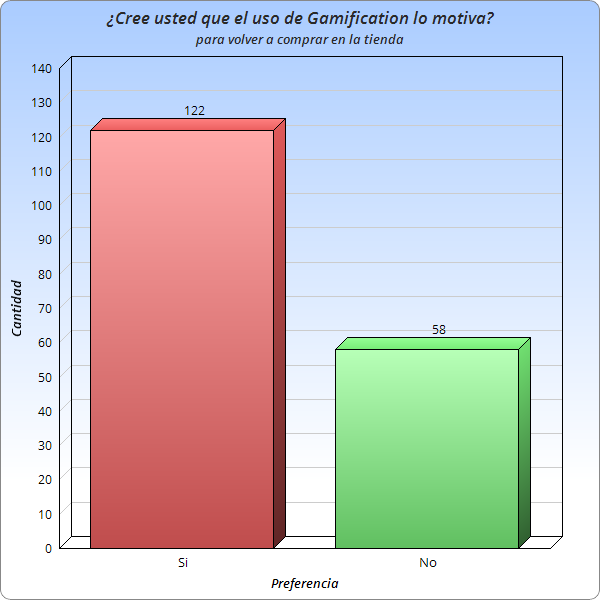
\includegraphics[width=0.6\textwidth]{images/Graficos/graf_5_11.png}
  \caption[chart5.11]{Respuesta a pregunta 10, motivación para volver a comprar en una misma tienda.}
  \label{fig:chart5.11}
  %\url{http://www.chartgo.com/get.do?id=69b1dc7d4e}
\end{figure}

\begin{figure}[!htb]
  \centering
  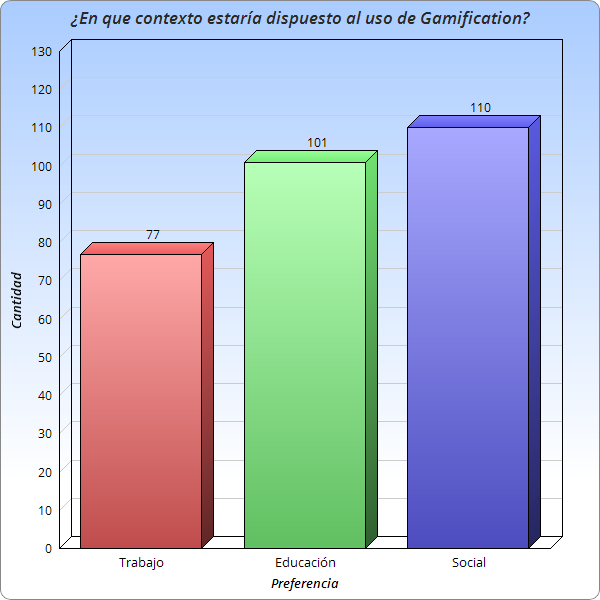
\includegraphics[width=0.6\textwidth]{images/Graficos/graf_5_12.png}
  \caption[chart5.12]{Respuesta a pregunta 11, contextos a los cuales se le podría implementar {\GAM}.}
  \label{fig:chart5.12}
  %\url{http://www.chartgo.com/get.do?id=69b1dc7d4e}
\end{figure}


